\documentclass[10pt]{article}
\date{}
\title{ELE2024 Lane Keeping Lab}
\author{Allwyn Bino}

\usepackage{gensymb}
\usepackage[left=2cm, right=2cm, top=1cm, bottom=2cm]{geometry}
\usepackage{graphicx}
\usepackage{float}
\usepackage{siunitx}
\usepackage{subfig}
\usepackage{amsmath}
\usepackage{amssymb}
\usepackage[outdir=../]{epstopdf}
\usepackage{inputenc}
\usepackage{sidecap}
\usepackage{caption}
\usepackage{hyperref}

\graphicspath{ {../Plots/} }
\sidecaptionvpos{figure}{c}
\hyphenpenalty=10000

\begin{document}
\maketitle

\section{Question 1}
The following graphs represent the dynamics of the car over $2\si{s}$. The steering angle is set to a constant $2\degree$. The length of the car is $2.3\si{m}$ and speed of the car is $5\si{m.s^{-1}}$. The initial starting conditions of the car was, $x_0 = 0\si{m}$, $y_0 = 0.3\si{m}$, $\theta_0$ = $5\degree$.

%\subsection{Question 1.1}
\begin{SCfigure}[1][h]
\centering
\includegraphics[width=11cm, height=8.25cm]{q1_x_t.eps}
\caption
{The x position of the car looks linear for the first $2\si{s}$ of its motion. But it is important to note, that it is not linear. The initial rotation is $5\degree$, the rotation after $2\si{s}$ is $-3.8\degree$. These values are sufficiently close to $0 \degree$, that it almost behaves as if $x$ is proportional to $t$. In reality \hyperref[3:x_prop]{x is proportional to $\sin(\theta)$}.}
\end{SCfigure}

\begin{SCfigure}[1][h]
\centering
\includegraphics[width=11cm, height=8.25cm]{q1_y_t.eps}
\caption
{The y position of the car doesn’t look linear, compared to the x position of the car. This is because \hyperref[3:y_prop]{y is proportional to $\cos(\theta)$}. $sin(0)$ isn’t close to the peak of the sinusoidal wave, whereas $cos(0)$ is the peak. The rate of change is greatest after the peak, so even small changes can have a noticeable outcome. Therefore, the y position has a noticeable change.}
\end{SCfigure}

\newpage
\begin{SCfigure}[1][h]
\centering
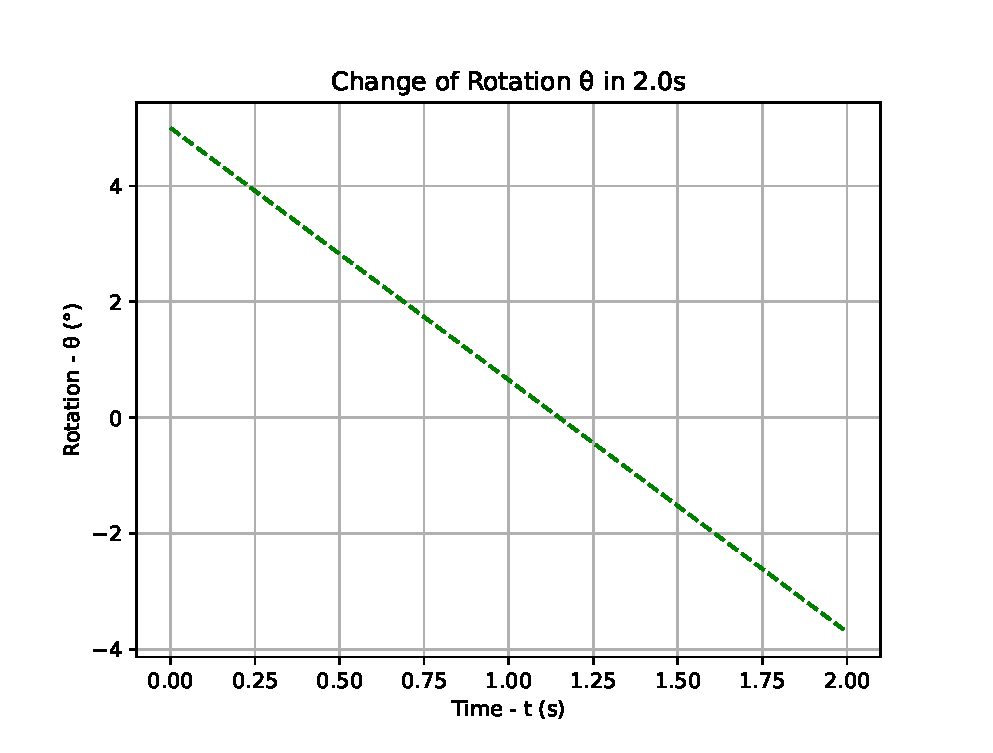
\includegraphics[width=11cm, height=8.25cm]{q1_theta_t.eps}
\caption
{The rotation of the car is linear. $\theta$ is directly proportional to time.}
\end{SCfigure}

%\subsection{Question 1.2}
\begin{SCfigure}[1][h]
\centering
\includegraphics[width=11cm, height=8.25cm]{q1Trajectory.eps}
\caption
{The trajectory traced by the car, isn’t recognisable from the first $2\si{s}$. But if it were simulated for about $80\si{s}$, it would be quite clear that its was tracing a circle. This is expected behaviour. If the car was moving with a constant speed at a constant steering angle, it would be expected to complete a circle.}
\end{SCfigure}

\newpage
\section{Question 2}
The following graphs represents the trajectory of a car of length $2.3\si{m}$ and constant velocity $5\si{ms^{-1}}$. The initial starting conditions of the car is $x_0 = 0\si{m}$, $y_0 = 0.3\si{m}$, $\theta_0 = 5\degree$. There is also a disturbance of 1\degree on the steering angle. The car was PID controlled. The sampling rate was $40\si{Hz}$.

%\subsection{Question 2.1}
\begin{SCfigure}[1][h]
\centering
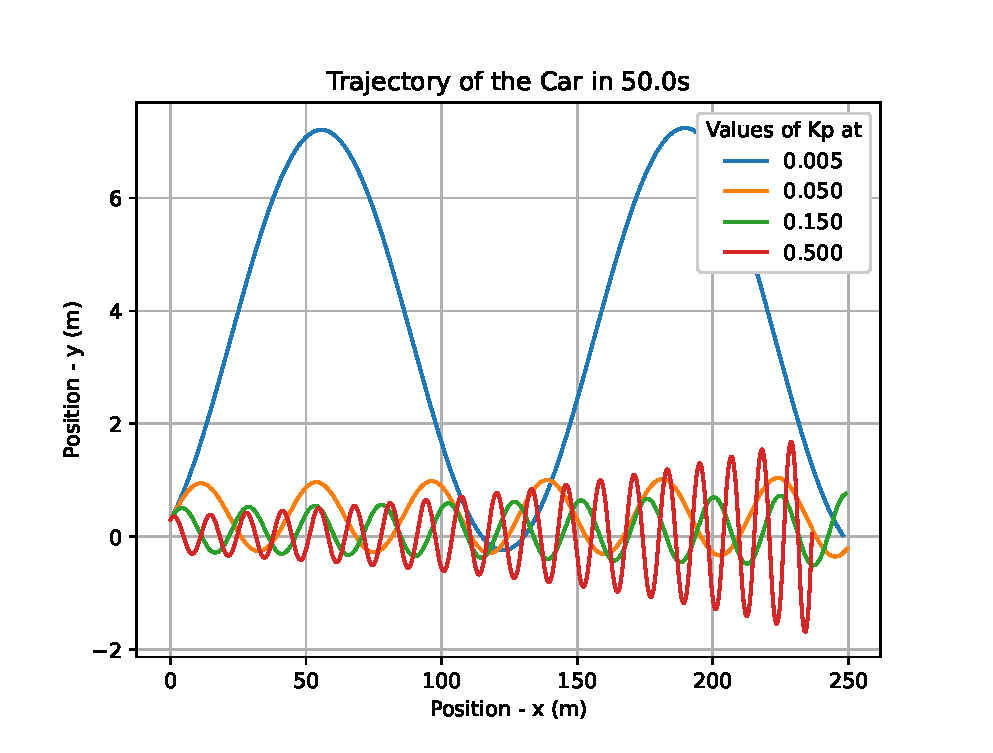
\includegraphics[width=11cm, height=8.25cm]{q2_1_trajectory.eps}
\caption
{This graph shows the car equipped with just a P Controller. The graph shows, that if the value of $K_p$ is small, it takes a much greater time to reach the setpoint. But it comes with the caveat that as $K_p$ is increased, the frequency of oscillation and amplitude of oscillation also increases. In general, as $K_p$ is increased, the time taken to reach the setpoint reduces.}
\end{SCfigure}

%\subsection{Question 2.2}
\begin{figure}[H]
\centering
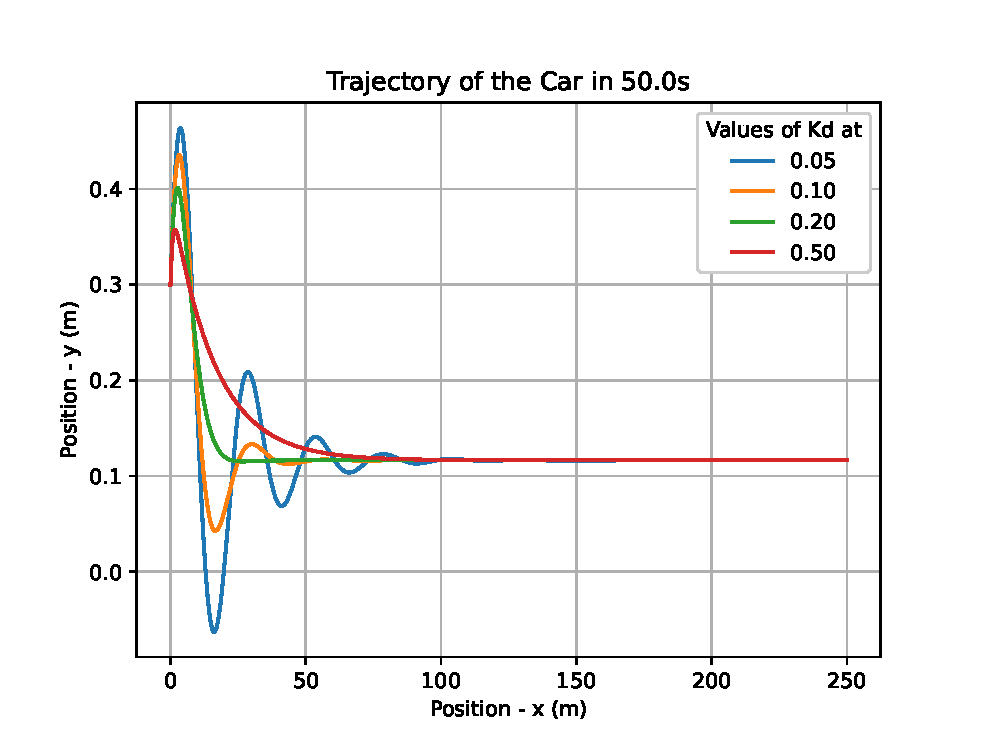
\includegraphics[width=11cm, height=8.25cm]{q2_2_trajectory.eps}
\caption
{This graph shows the car equipped with a PD Controller. The value of $K_p$ is fixed at 0.15. The graph shows, that as $K_d$ is increased the frequency of oscillation starts to decrease, by decreasing amplitude faster. An important point about the PD controller, is that the system eventually settles at an equilibrium position. The equilibrium position doesn’t have to be the setpoint. In this case, the equilibrium position isn’t the setpoint. If the value of $K_d$ is set too high, the oscillations cease, but the time taken to reach the equilibrium position increases. In general, as $K_d$ is increased, the oscillations and time taken to reach the equilibrium position decreases. But after a certain value of $K_d$, there is no oscillation, but the time taken to reach the equilibrium position increases.}
\end{figure}

\newpage
%\subsection{Question 2.3}
For the following graphs, $K_p$ = 0.15, $K_d$ = 0.2, and $K_i$ = 0.02. These values were chosen, because they allowed the car to reach the setpoint fastest, with no oscillations.

\begin{figure}[H]
\centering
\includegraphics[width=11cm, height=8.25cm]{q2_3i_u_t.eps}
\caption
{This graph shows how steering angle changes with time. Initially, the steering angle is at $-2.5\degree$. Then it is turned to a $-7.5\degree$, and then quickly increased. Then when the car is close enough to the setpoint, it starts to decrease the steering angle, until it settles on a value of $-1\degree$. This $-1\degree$ value makes sense, as there is a disturbance on the car of $1\degree$. To stay on the setpoint, the rotation of the car has to be $0\degree$. So the $-1\degree$ steering angle is needed to accommodate for the disturbance and ensure no further rotation of the car.}
\end{figure}

\begin{figure}[H]
\centering
\subfloat[\centering Perfect Values]{{\includegraphics[width=8cm, height=6cm]{q2_3ii_trajectory.eps}}}
\qquad
\subfloat[\centering Varying $K_i$ Values]{{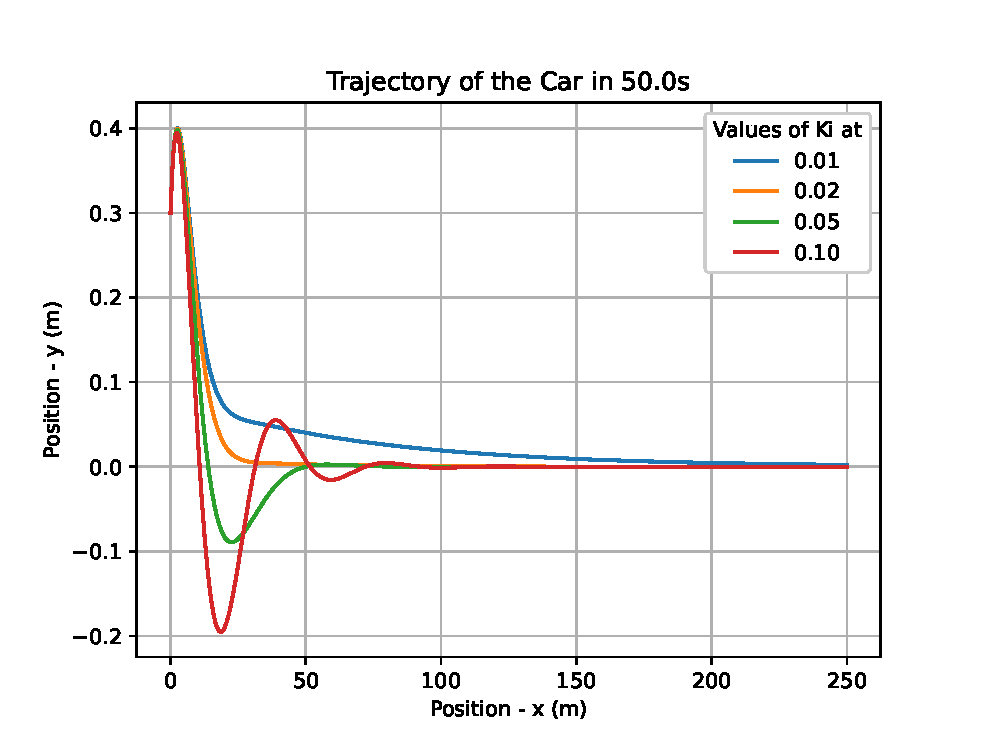
\includegraphics[width=8cm, height=6cm]{q2_3ii_trajectory2.eps}}}
\caption
{(a) This graph shows the trajectory of the car with ideal $K_p$, $K_d$, and $K_i$ values. These are 0.15, 0.2, 0.02 respectively.\\
(b) This graph shows the car equipped with a PID controller. The value of $K_p = 0.15$ and $K_d = 0.2$. It shows that, in general $K_i$ is introduced to ensure the system converges to the setpoint, and not the offset. As $K_i$ is increased, the system reaches the setpoint faster. But after a certain value of $K_i$, an increase in $K_i$ can reintroduce oscillations.}
\end{figure}

%\newpage
%\subsection{Question 2.4}
\begin{SCfigure}[1][h]
\centering
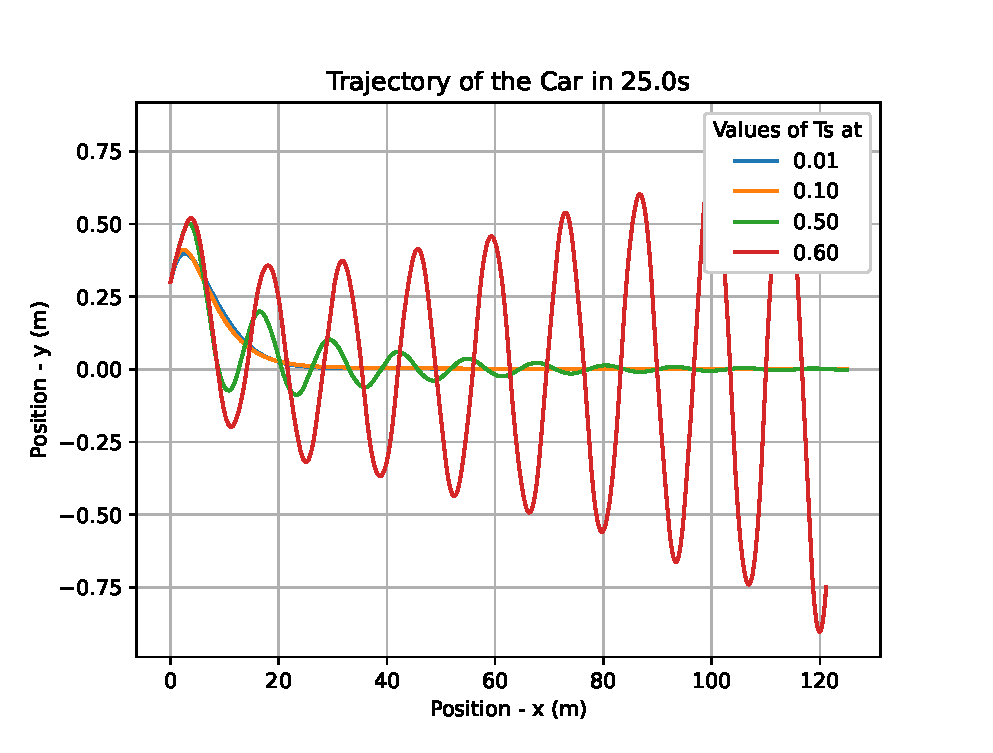
\includegraphics[width=11cm, height=8.25cm]{q2_4_trajectory.eps}
\caption
{This graph show how sampling time can affect the performance of the car. Below a certain value of sampling time, (threshold time) a decrease in sampling time doesn’t affect performance. On the other hand, increasing sampling time after this threshold time affects performance poorly. 
This is because, when the PID Controller samples the error at a certain point in time, the output it produces is only valid for a certain amount of time. The reason for this, is that the car is moving, therefore producing a new error. If the sampling time is greater than this threshold time, then the system will never be able produce the correct output at the correct time to bring the system to the setpoint.
}
\end{SCfigure}

\section{Question 3}

\begin{equation*}
\dot{Z} = 
\begin{bmatrix}
\dot{x}\cr
\dot{y}\cr
\dot{\theta}\cr
\end{bmatrix}
=
\begin{bmatrix}
v\cos(\theta)\cr
v\sin(\theta)\cr
\frac{v}{L}\tan(u)\cr
\end{bmatrix}
\end{equation*}

\[\frac{d\theta}{dt} = \frac{v}{L}\tan(u)\]
\[\int \frac{d\theta}{dt}\,dt = \int \frac{v}{L}\tan(u)\,dt \]
\[\theta = \frac{v}{L}\tan(u)t + c\]
\[\theta = \frac{v}{L}\tan(u)(0) + c\]
\[\theta(0) = \theta_0 = c\]
\[\therefore \theta = \frac{v}{L}\tan(u)t + \theta_0\]\\


\[\frac{dx}{dt} = v\cos(\theta)\]
\[\frac{dx}{dt} = v\cos(\frac{v}{L}\tan(u)t + \theta_0)\]
\[\int \frac{dx}{dt}\, dt = \int v\cos(\frac{v}{L}\tan(u)t + \theta_0)\, dt\]
\[x= \frac{L}{\tan{u}}\sin(\frac{v}{L}\tan(u)t + \theta_0) + d\]
\[x(0)= \frac{L}{\tan{u}}\sin(\frac{v}{L}\tan(u)(0) + \theta_0) + d\]
\[x(0)= x_0 = \frac{L}{\tan{u}}\sin(\theta_0) + d\]
\[d = x_0 - \frac{L}{\tan{u}}\sin(\theta_0)\]
\[\therefore x= \frac{L}{\tan{u}}\sin(\theta) - \frac{L}{\tan{u}}\sin(\theta_0) + x_0\]\\
\label{3:x_prop}

\[\frac{dy}{dt} = v\sin(\theta)\]
\[\frac{dy}{dt} = v\sin(\frac{v}{L}\tan(u)t + \theta_0)\]
\[\int \frac{dy}{dt}\, dt = \int v\sin(\frac{v}{L}\tan(u)t + \theta_0)\, dt\]
\[y = \frac{-L}{\tan{u}}\cos(\frac{v}{L}\tan(u)t + \theta_0) + f\]
\[y(0) = \frac{-L}{\tan{u}}\cos(\frac{v}{L}\tan(u)(0) + \theta_0) + f\]
\[y(0)= y_0 = \frac{-L}{\tan{u}}\cos(\theta_0) + f\]
\[f = y_0 + \frac{L}{\tan{u}}\cos(\theta_0)\]
\[\therefore y= \frac{-L}{\tan{u}}\cos(\theta) + \frac{L}{\tan{u}}\cos(\theta_0) + y_0\]\\
\label{3:y_prop}

\begin{equation*}
Z = 
\begin{bmatrix}
x\\
y\\
\theta
\end{bmatrix}
=
\begin{bmatrix}
\frac{L}{\tan{u}}\sin(\theta) - \frac{L}{\tan{u}}\sin(\theta_0) + x_0\cr
\frac{-L}{\tan{u}}\cos(\theta) + \frac{L}{\tan{u}}\cos(\theta_0) + y_0\cr
\frac{v}{L}\tan(u)t + \theta_0\cr
\end{bmatrix}
\end{equation*}

\bigskip
\noindent
For $x_0 = 0\si{m}$, $y_0 = 0\si{m}$, the input values, scipy's solve\_ivp answers, and the calculated values are shown. \\
Note: All $\theta_0$ values have been fixed to the range, $(-180\degree, 180\degree]$, and only correct to 3sf. \\
%\bigskip

\begin{center}
\begin{tabular}{| c c c c | c c c | c c c |}
\hline
\multicolumn{4}{| c |}{Variables} & \multicolumn{3}{c |}{solve\_ivp Values} & \multicolumn{3}{c |}{Calculated Values} \\ \hline
L & v & u & $\theta_0$ & x & y & $\theta$ & x & y & $\theta$ \cr \hline
2.3 & 5 & -2 & 5 & -29.628 & -121.174 & 147.520 & -29.628 & -121.174 & 147.520\cr
2.5 & 5 & -10 & 20 & -9.329 & -13.254 & 89.721 & -9.329 & -13.254 & 89.721\cr
5 & 10 & -30 & 40 & 9.629 & 1.014 & -27.973 & 9.629 & 1.014 & -27.973\cr
5 & 5 & -60 & 40 & -0.692 & -3.568 & 118.040 & -0.692 & -3.568 & 118.040\cr
10 & 10 & -60 & 40 & -1.385 & -7.137 & 118.040 & -1.385 & -7.137 & 118.040\cr
\hline
\end{tabular}
\end{center}

\bigskip
\noindent
From the table, it is clear that solve\_ivp values and calculated value are identical.


\end{document}